\documentclass{crypto-exercise}
\usepackage{amsthm}
\usepackage{float}
\usepackage{pgfplots}
\usepackage{tikz}

\author{Sven Laur}
\contributor{Sander Siim}
\editor[Redrawed figures to Tikz]{Sven Laur}
\tags{hypothesis testing, false positives, false negatives, tradeoff}


\begin{document}
\begin{exercise}{Convex closure for distinguishers}
Let $\AD$ and $\ADB$ be a $t$-time distinguishers with the following ratios for false negatives and false positives:
\begin{align*}
&\begin{aligned}
\alpha(\AD) &= \pr{\AD(x) = 0|\HHH_1}\\
\alpha(\ADB) &= \pr{\ADB(x) = 0|\HHH_1}
\end{aligned} &
&\begin{aligned}
\beta(\AD) &= \pr{\AD(x) = 1 | \HHH_0}\\
\beta(\ADB) &= \pr{\ADB(x) = 1 | \HHH_0}
\end{aligned}
\end{align*}
Show that for any $\lambda\in[0,1]$ there exists a $t + O(1)$-time adversary $\ADC$ such that
\begin{align*}
\alpha(\ADC) &= \lambda \cdot \alpha(\AD) + (1-\lambda)\cdot\alpha(\ADB)\enspace,\\
\beta(\ADC)  &= \lambda \cdot \beta(\AD) + (1-\lambda)\cdot\beta(\ADB)\enspace.
\end{align*}
Explain the consequences of this result by sketching the region of achievable tradeoffs on the false negative $\alpha(\cdot)$ and false positive $\beta(\cdot)$ plane for many tradeoffs.  
\end{exercise}
\begin{solution}

Let us first construct the required distinguisher $\ADC$. The construction is as follows:
\begin{align*}
    \begin{fblock}{\ADC_{\lambda}(x)}
    & \lambda_* \getsu [0,1]\\
    & \IF \lambda_* \leq \lambda \hspace{2pt} \THEN \RETURN \AD(x)\\
    &  \RETURN \ADB(x) \enspace.
    \end{fblock}     
\end{align*}
As we first sample $\lambda_*$ uniformly from the range $[0,1]$, the distinguisher returns the output of $\AD$ on the given input $x$ with probability exactly $\lambda$. Otherwise, the output of $\ADB(x)$ is returned instead, with probability $1- \lambda$. Let us  ratios for false positives and false negatives for $\ADC$. For false negatives, we get
\begin{align*}
\alpha(\ADC) &= \pr{\ADC(x) = 0 | \HHH_1}\\
 &= \pr{\lambda_* \leq \lambda}\cdot\pr{\AD(x) = 0 | \HHH_1} + \pr{\lambda_* > \lambda}\cdot\pr{\ADB(x) = 0 | \HHH_1}\\
 &= \lambda\cdot\pr{\AD(x) = 0 | \HHH_1} + \left(1 - \lambda\right)\cdot\pr{\ADB(x) = 0 | \HHH_1}\\
 &= \lambda \cdot \alpha(\AD) + \left(1-\lambda\right)\cdot\alpha(\ADB)\enspace
\end{align*}
which is exactly the required ratio. Similarly, for false positives:
\begin{align*}
\beta(\ADC) &= \pr{\ADC(x) = 1 | \HHH_0}\\
 &= \pr{\lambda_* \leq \lambda}\cdot\pr{\AD(x) = 1 | \HHH_0} + \pr{\lambda_* > \lambda}\cdot\pr{\ADB(x) = 1 | \HHH_0}\\
 &= \lambda\cdot\pr{\AD(x) = 1 | \HHH_0} + \left(1 - \lambda\right)\cdot\pr{\ADB(x) = 1 | \HHH_0}\\
 &= \lambda \cdot \beta(\AD) + \left(1-\lambda\right)\cdot\beta(\ADB)\enspace
\end{align*}
Thus, this construction achieves the required ratios for false positives and negatives for any $\lambda\in[0,1]$.


Let us now analyse the running time of $\ADC$. The distinguisher needs to sample a random value from $[0,1]$, do one comparison and then call either $\AD$ or $\ADB$. For obvious reason, it is not possible to sample real numbers with ordinary computers. Hence, this step is actually approximated by sampling $n$ random coin-flips and consequently we achieve only tradeoff points $\lambda\in\set{0, 2^{-n}, 2\cdot 2^{-n},\ldots, 2^n\cdot 2^{-n}}$. As a result, the running time of $\ADC$ is clearly $t + O(n)$ whenever the running times of $\AD$ and $\ADB$ are below $t$. Note that the precision grows exponentially with the parameter $n$ and thus achieving desired precision is not a practical problem.  

Intuitively, this result shows that it is always possible to combine distinguishers $\AD$ and $\ADB$ such that the resulting distinguisher $\ADC$ has averaged false positive and false negative ratios. If the ratios of false negatives and false positives differ, then it is possible to seek different balance points between. Figure~\ref{fig:tradeoffs-i} visualises basic properties of such tradeoffs. Each distinguisher can be viewed as a point in the false negative false positive plane. Achievable tradeoffs are on the line between $\AD$ and $\ADB$. Black segments on the axis show achievable trade-off regions for false negatives and for false positives, respectively. Dash-dotted diagonal lines show equilines for aggregate error $\gamma$. For obvious reasons the aggregate error of the tradeoff is always larger than the aggregate error of the better distinguisher. In other words, the increase in false positives is always larger than the decrease in false negatives and vice versa. The only exception to this rule is the setting where both distinguishers have the same aggregate error. In this case, the tradeoff is the zero sum game.  

\begin{figure}[H]
\begin{center} 
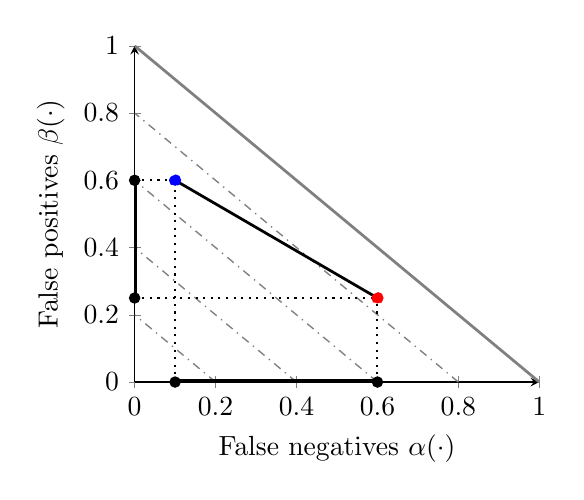
\begin{tikzpicture}
\begin{axis}[
	scale=0.75,
    axis x line =bottom,  % only show the bottom x axis line, without an arrow tip
    axis y line =left,
    xmin=0, xmax=1,  % range for the x axis
    ymin=0, ymax=1, 
    xlabel = {False negatives $\alpha(\cdot)$},
    ylabel = {False positives $\beta(\cdot)$},
]
\addplot [gray, line width=1pt, style={solid}]
	coordinates {(1.0, 0.0) (0.0, 1.0)};	
\addplot [gray, line width=0.5pt, style={dashdotted}]
	coordinates {(0.8, 0.0) (0.0, 0.8)};	
\addplot [gray, line width=0.5pt, style={dashdotted}]
	coordinates {(0.6, 0.0) (0.0, 0.6)};	
\addplot [gray, line width=0.5pt, style={dashdotted}]
	coordinates {(0.4, 0.0) (0.0, 0.4)};	
\addplot [gray, line width=0.5pt, style={dashdotted}]
	coordinates {(0.2, 0.0) (0.0, 0.2)};	

\addplot+[only marks, mark=*, mark options={blue}] 
	coordinates {(0.1, 0.6)}
	[yshift=10pt, black]
	node[pos=0]{$\AD$}
;	
\addplot+[only marks, mark=*, mark options={red}] 
	coordinates {(0.6, 0.25)}
	[yshift=10pt, black]
	node[pos=0]{$\ADB$}
;	
\addplot [black, line width=1pt]
	coordinates {(0.1, 0.6) (0.6, 0.25)}
;	
\addplot [black, line width=2pt, mark=*, mark size=1pt]
	coordinates {(0.1, 0.0) (0.6, 0.0)}
;	
\addplot [black, line width=0.75pt, style={dotted}]
	coordinates {(0.1, 0.0) (0.1, 0.6)}
;	
\addplot [black, line width=0.75pt, style={dotted}]
	coordinates {(0.6, 0.0) (0.6, 0.25)}
;	
\addplot [black, line width=2pt, mark=*, mark size=1pt]
	coordinates {(0.0, 0.25) (0.0, 0.6)}
;	
\addplot [black, line width=0.75pt, style={dotted}]
	coordinates {(0.0, 0.25) (0.6, 0.25)}
;	
\addplot [black, line width=0.75pt, style={dotted}]
	coordinates {(0.0, 0.6) (0.1, 0.6)}
;	
\end{axis}
\end{tikzpicture} 
\hspace*{2cm}
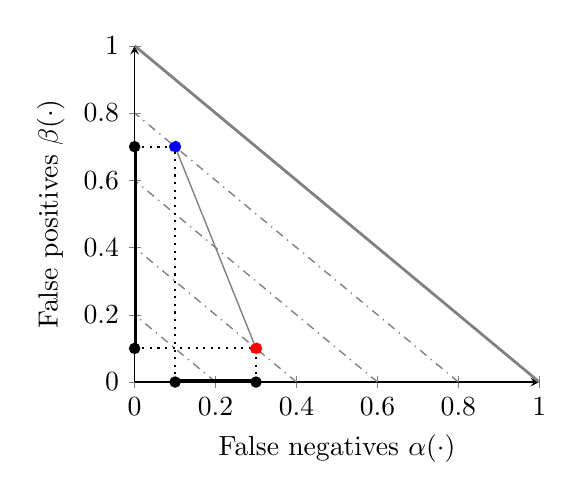
\begin{tikzpicture}
\begin{axis}[
	scale=0.75,
    axis x line =bottom,  % only show the bottom x axis line, without an arrow tip
    axis y line =left,
    xmin=0, xmax=1,  % range for the x axis
    ymin=0, ymax=1, 
    xlabel = {False negatives $\alpha(\cdot)$},
    ylabel = {False positives $\beta(\cdot)$},
]
\addplot [gray, line width=1pt, style={solid}]
	coordinates {(1.0, 0.0) (0.0, 1.0)};	
\addplot [gray, line width=0.5pt, style={dashdotted}]
	coordinates {(0.8, 0.0) (0.0, 0.8)};	
\addplot [gray, line width=0.5pt, style={dashdotted}]
	coordinates {(0.6, 0.0) (0.0, 0.6)};	
\addplot [gray, line width=0.5pt, style={dashdotted}]
	coordinates {(0.4, 0.0) (0.0, 0.4)};	
\addplot [gray, line width=0.5pt, style={dashdotted}]
	coordinates {(0.2, 0.0) (0.0, 0.2)};	

\addplot+[only marks, mark=*, mark options={blue}] 
	coordinates {(0.1, 0.7)}
	[yshift=10pt, black]
	node[pos=0]{$\AD$}
;	
\addplot+[only marks, mark=*, mark options={red}] 
	coordinates {(0.3, 0.1)}
	[yshift=10pt, xshift=3pt, black]
	node[pos=0]{$\ADB$}
;	
\addplot [gray, line width=0.5pt]
	coordinates {(0.1, 0.7) (0.3, 0.1)}
;	
\addplot [black, line width=2pt, mark=*, mark size=1pt]
	coordinates {(0.1, 0.0) (0.3, 0.0)}
;	
\addplot [black, line width=0.75pt, style={dotted}]
	coordinates {(0.1, 0.0) (0.1, 0.7)}
;	
\addplot [black, line width=0.75pt, style={dotted}]
	coordinates {(0.3, 0.0) (0.3, 0.1)}
;	
\addplot [black, line width=2pt, mark=*, mark size=1pt]
	coordinates {(0.0, 0.1) (0.0, 0.7)}
;	
\addplot [black, line width=0.75pt, style={dotted}]
	coordinates {(0.0, 0.1) (0.3, 0.1)}
;	
\addplot [black, line width=0.75pt, style={dotted}]
	coordinates {(0.0, 0.7) (0.1, 0.7)}
;	
\end{axis}
\end{tikzpicture} 

\end{center}

\caption{Nature of tradeoff between two distinguishers $\AD$ and $\ADB$}
\label{fig:tradeoffs-i}
\end{figure}

Same principles apply if there are many distinguishers to choose from. However, not all of them are useful, as tradeoffs between different distinguishers might have better parameters. Figure~\ref{fig:distinguishing-profile} describes a distinguishing profile where some classifiers are useless. As there are trivial distinguishers with parameters $(0,1)$ and $(1,0)$ and distinguishers with aggregate error $\gamma>1$ can be inverted to improve aggregate error, the distinguishing profile is a convex-cup line below the line $\alpha+\beta=1$. Since the lower bound on aggregate error is determined by statistical distance, the distinguishing profile must be above $\alpha+\beta=1-\SD(\XXX_0,\XXX_1)$. For the same reason the closest point to the corner on the profile determines the computational distance $\CD_x^t(\XXX_0,\XXX_1)$.   

\begin{figure}[H]
\begin{center}
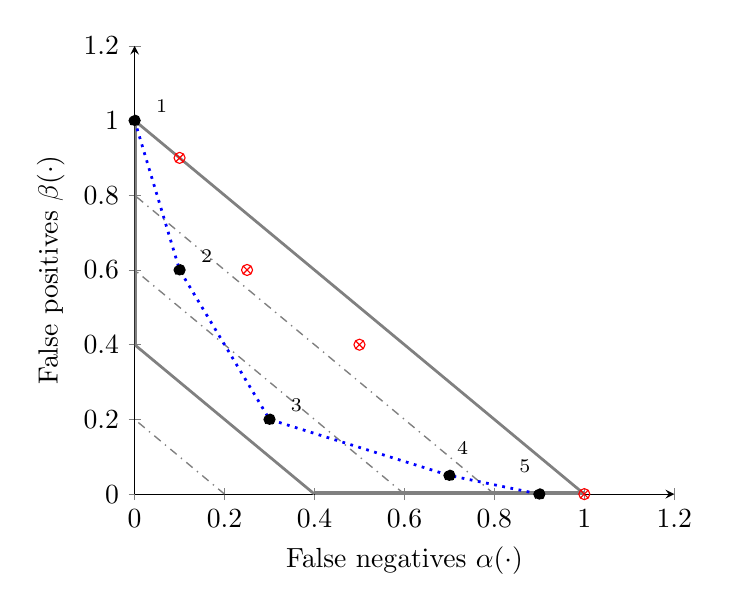
\begin{tikzpicture}
\begin{axis}[
	scale=1.00,
    axis x line =bottom,  % only show the bottom x axis line, without an arrow tip
    axis y line =left,
    xmin=0, xmax=1.2,  % range for the x axis
    ymin=0, ymax=1.2, 
    xlabel = {False negatives $\alpha(\cdot)$},
    ylabel = {False positives $\beta(\cdot)$},
]
\addplot [gray, line width=1pt, style={solid}]
	coordinates {(1.0, 0.0) (0.0, 1.0)};	
\addplot [gray, line width=0.5pt, style={dashdotted}]
	coordinates {(0.8, 0.0) (0.0, 0.8)};	
\addplot [gray, line width=0.5pt, style={dashdotted}]
	coordinates {(0.6, 0.0) (0.0, 0.6)};	
\addplot [gray, line width=1.pt, style={solid}]
	coordinates {(0.4, 0.0) (0.0, 0.4)};	
\addplot [gray, line width=0.5pt, style={dashdotted}]
	coordinates {(0.2, 0.0) (0.0, 0.2)};	
\addplot [gray, line width=2pt, style={solid}]
	coordinates {(0.4, 0.0) (1.0, 0.0)};	
\addplot [gray, line width=2pt, style={solid}]
	coordinates {(0.0, 0.4) (0.0, 1.0)};	

\addplot+[only marks, mark=*, mark options={black}] 
	coordinates {(0, 1)(0.1, 0.6) (0.3, 0.2 ) (0.7, 0.05) (0.9, 0)}
	[black]
	node[pos=0.00, xshift=10pt, yshift=5pt]{$\AD_1$}
	node[pos=0.25, xshift=10pt, yshift=5pt]{$\AD_2$}
	node[pos=0.50, xshift=10pt, yshift=5pt]{$\AD_3$}
	node[pos=0.75, xshift= 5pt, yshift=10pt]{$\AD_4$}
	node[pos=1.00, xshift=-5pt, yshift=10pt]{$\AD_5$}
;	
\addplot [color=blue, line width=1.0pt, style={dotted}] 
	coordinates {(0, 1)(0.1, 0.6) (0.3, 0.2 ) (0.7, 0.05) (0.9, 0)}
;	

\addplot [only marks, mark=otimes, color=blue, color=red] 
	coordinates {(0.1, 0.9) (0.25, 0.6) (0.5, 0.4) (1.0, 0)}
;	



%
\end{axis}
\end{tikzpicture} 
\end{center}
\caption{Distinguishing profile is nearly convex-cup line as all distinguishes worse than the averages of distinguisher pairs should be discarded. Discrepancies form convex-cup line are caused by running time constraints. The higher the the bound on the running time is the closer to the corner the profile moves. At limit it is completely determined by the likelihood ratio test.}
\label{fig:distinguishing-profile}
\end{figure}

\end{solution}
\end{document}